\input{settings}
\setlength{\emergencystretch}{2em}
\titleformat{\section}
  {\small\bfseries\raggedright}
  {}{0em}
  {}
  [{\color{WHU_Blue}\titlerule}]
\titlespacing*{\section}{0cm}{0.85em}{0.60em}
\titlespacing*{\subsection}{0cm}{0.50em}{0.30em}
\setlist[itemize]{topsep=0.20em, itemsep=0.20em, parsep=0em, partopsep=0em, leftmargin=1.25em}
\setlist[enumerate]{topsep=0.20em, itemsep=0.20em, parsep=0em, partopsep=0em, leftmargin=1.35em}
\renewcommand{\arraystretch}{0.98}
\renewcommand{\CJKglue}{\hskip 0.018em}

% 个人信息
%  cd C:\Users\31087\Documents\Obsidian_Vault\Resume\template
%  xelatex main_general.tex
\newcommand{\school}{江南大学 · 控制科学与工程}

\newcommand{\resumeDecor}{
    \begin{tikzpicture}[remember picture, overlay]
        \node[anchor=north, inner sep=0pt](header) at (current page.north){
            
\includegraphics[width=\paperwidth]{images/header.png}
        };
        \node[anchor=west](school_logo) at (header.west){
            \hspace{0.5cm}
            
\includegraphics[width=0.15\textwidth]{images/whu_logo_1.png}
        };
        \node[anchor=east](school_name) at(header.east){
            \textcolor{white}{\textbf{\school}}
            \hspace{0.5cm}
        };
    \end{tikzpicture}

    \begin{tikzpicture}[remember picture, overlay]
        \node[opacity=0.05] at(current page.center){
            
\includegraphics[width=0.68\paperwidth, keepaspectratio]{images/whu_logo_big.png}
        };
    \end{tikzpicture}
}

\newcommand{\sectionIcon}[2]{\makebox[\widthof{#1}][c]{\color{WHU_Blue}{#1}}\quad #2}

%%%%%%%%%%%%%%%%%%%%
% 简历正文
% cd template && xelatex -interaction=nonstopmode main_general.tex && xelatex -interaction=nonstopmode main_general.tex
%%%%%%%%%%%%%%%%%%%%
\begin{document}
\resumeDecor
\vspace*{-3.15em}
\scriptsize
\linespread{1.10}\selectfont

\begin{minipage}{0.80\textwidth}
    \section[个人信息]{\sectionIcon{\faAddressCard}{个人信息}}
    \footnotesize
    \begin{tabularx}{\linewidth}{p{\widthof{求职意向:}}Xp{\widthof{最高学历:}}X}
        姓\ \ \ \ \ \ \ \ 名: & 梁邦一 &
        性\ \ \ \ \ \ \ \ 别: & 男 \\
        邮\ \ \ \ \ \ \ \ 箱: & yuejinai55@gmail.com &
        电\ \ \ \ \ \ \ \ 话: & +86 15515602693 \\
        英语等级: & CET-6 &
        求职意向: & 研发类；感知算法、AI 应用、具身智能 \\
    \end{tabularx}
\end{minipage}
\hfill
\begin{minipage}{0.11\textwidth}
    \vspace{2.0em}
    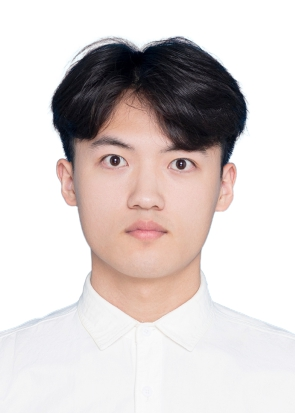
\includegraphics[width=\linewidth]{images/avatar.png}
\end{minipage}
\vspace{-0.60em}

% \section[个人总结]{\sectionIcon{\faBook}{个人总结}}
% 控制科学与工程硕士在读，本科自动化背景，具备 Python / PyTorch / Linux / ROS2 和机器人实验联调基础。参与过感知数据挖掘、机器人感知训练复现与端侧部署、Linux 服务器环境搭建和 PLC 设备优化，能够在数据处理、模型实验、系统联调和文档交付中快速上手。长期参与班级和实验室协作，沟通推进意识较强，适合技术类校招岗位。

\section[教育背景]{\sectionIcon{\faGraduationCap}{教育背景}}
\begin{itemize}
    \item {\textbf{控制科学与工程硕士，江南大学}}（\hl{中国科学院沈阳自动化研究所 · 机器人与智能系统全国重点实验室联合培养}） \hfill {2024.06--2027.06}
    \item {\textbf{自动化学士，郑州轻工业大学}} \hfill {2020.09--2024.06}
\end{itemize}

\section[荣誉与组织经历]{\sectionIcon{\faStar}{荣誉与组织经历}}
\begin{itemize}
    \item {\textbf{荣誉奖项}}：中国机器人大赛暨 RoboCup 机器人世界杯中国赛 \hl{国家三等奖}；校一等奖学金（2025.10、2026）；优秀毕业生（2024.06）；优秀班干部（2022.10）。
    \item {\textbf{组织经历}}：本科班长（2020.10-2024.06）；硕士党支部书记（2024.10-2026.05），具备跨角色沟通、任务分解和协作推进经验。
\end{itemize}

\section[专业技能]{\sectionIcon{\faWrench}{专业技能}}
\begin{itemize}
    \item \textbf{算法与模型}：Python、C++、PyTorch、Transformer、轻量级 Conformer、YOLO11s-seg、目标检测、实例分割、分类、连续值回归、时序建模、多模态特征融合。
    \item \textbf{端侧部署}：TensorRT、ONNX、NVIDIA Jetson AGX Orin、模型量化与算子优化。
    \item \textbf{机器人与仿真}：ROS2（Python / C++）、Topic 通信、灵巧手遥操作、机器人端联调、MuJoCo、Gazebo。
    \item \textbf{数据工程}：视觉/多通道数据清洗标注、训练/验证/测试集划分、vLLM 批量推理、JSON 标签解析、bad case 归因。
    \item \textbf{工程环境}：Linux / Ubuntu、Git、bash、LLaMA-Factory、代码仓库与运行文档管理。
\end{itemize}


\vspace{0.04em}
\section[实习经历]{\sectionIcon{\faBriefcase}{实习经历}}
{\small\textbf{CARIZON（大众×地平线合资智驾）}}\quad 感知数据部门算法实习生 \hfill {2026.06--至今} \\
{\scriptsize\color{WHU_Blue} 感知数据闭环 / VLM 后训练 / 长尾场景挖掘}
\begin{itemize}
    \item 设计红绿灯自车转向挖掘 Tagger，融合车载多路传感器与回灌数据设计规则化挖掘算子，在 3W 条路口数据中筛选 3K 条转向 CLIP，\hl{标签验收准确率达 90\%、挖掘召回提升 10\%}；梳理 Grounding DINO、GDINO + VLM、tagger 配置到模型 worker 的调用链，沉淀模型选型与工程排查文档。
    \item 负责泊车障碍物识别 VLM 优化，筛选 1.8 万张挡轮杆图像完成数据清洗、标注校验与 Prompt 迭代，基于 Qwen3-VL-8B + LLaMA-Factory \hl{在 4 机 8 卡 H20 完成全参数 SFT}；针对类别误判等验收问题设计基于 GRPO 的三元组策略优化，完成模型二次精标业务交付。
    \item 针对实车难覆盖的废弃地面箭头、引导线等 Corner Case，设计“规则渲染 + 生成模型”合成 pipeline，\hl{生成 5K 张高质量训练样本}，填补实车采集空白，支撑挖掘模型冷启动迭代。
\end{itemize}

\vspace{0.30em}
{\small\textbf{优奇智能科技有限公司（优必选子公司）}}\quad 人形机器人感知算法实习生 \hfill {2026.02--2026.05} \\
{\scriptsize\color{WHU_Blue} 端侧部署与推理加速 / 目标检测与实例分割 / 数据质检}
\begin{itemize}
    \item 负责 R11 接待机器人感知模型在 NVIDIA Jetson AGX Orin 端侧计算平台的部署，围绕 TensorRT 完成 PyTorch $\rightarrow$ ONNX $\rightarrow$ TensorRT 模型转换、量化与算子性能优化，\hl{推理延迟降低 20\%}，在真机跑通检测/分割实时推理链路。
    \item 参与 R11 接待机器人 YOLO11s-seg 模型训练复现与多场景数据质检、训练/验证/测试集划分，\hl{推动检测/分割训练链路跑通}；面向真实机器人场景归纳误检、漏检与分割边界不稳定等 bad case，\hl{将模型效果问题转化为可执行的数据侧优化需求}。
\end{itemize}

\section[科研与项目经历]{\sectionIcon{\faFlask}{科研与项目经历}}
{\small\textbf{面向具身智能灵巧操作的肌电-力融合感知与灵巧手抓取控制系统（灵心巧手） · 负责人}} \hfill {2025.02--2026.02}\\
{\scriptsize\color{WHU_Blue} 承载平台：中国科学院沈阳自动化研究所 · 机器人与智能系统全国重点实验室（江南大学联合培养）}
\begin{itemize}
    \item 搭建视觉 + Delsys Trigno sEMG + Sensel 压力多模态同步采集链路，完成抓取任务配置、会话标注、CSV 落盘与实时可视化，\hl{形成可复现实验数据入口}；基于 PyTorch 推进 Transformer / 轻量 Conformer 肌电—力映射实验，支持\hl{力等级分类与连续力值回归双任务}。
    \item 设计视觉—MuJoCo—sEMG—触觉分层控制链路，通过 ROS2 对接 Linker Hand G20 并沉淀模块化接口，使视觉、仿真策略、肌电力估计与触觉控制模块能够独立替换、调试和验证，构成 \hl{Sim-to-Real 端到端方案雏形}。
    \item 负责课题实验链路组织与 \hl{Linux 训练服务器搭建维护}，完成传感器准备、通道配置、训练配置管理和结果检查，保障多轮实验数据可追溯、可复查。
    \item 系统性梳理手势识别、人机交互与机器人感知方向英文文献，归纳传感器方案、算法框架、数据集与应用场景，\hl{支撑综述论文写作}、课题选型与技术路线判断。
\end{itemize}

\section[论文与研究成果]{\sectionIcon{\faBook}{论文与研究成果}}
三篇工作构成\hl{「综述定路线 — 算法破难点 — 系统做闭环」}的完整研究链条：
\begin{itemize}
    \item \hl{已中（JCR 一区 / 中科院二区）} Liang B., Li N., Li G., et al. \textit{Sensing Technologies for Hand Gesture Recognition in Human-Robot Interaction: A Review}. IEEE Sensors Journal, 2025, 26(2): 1501-1519. \textbf{综述}：梳理数据手套、视觉与肌电等手势感知路线，对比精度、侵入性与成本取舍。
    \item \hl{在修（JCR 一区 / 中科院二区 Top）} \textit{sEMG Conformer: Synergizing Local-Global Spatiotemporal Features for Continuous Force Estimation}. Biomedical Signal Processing and Control. \textbf{算法核心}：卷积局部感受野 + 自注意力全局建模，解码肌电—指尖力映射，单模型支持力等级分类与连续力值回归。
    \item \hl{在投（JCR 一区 / 中科院二区）} \textit{Dexterous Hand Grasping Control Based on Multimodal Sensory Fusion and Simulation Reinforcement Learning}. \textbf{系统闭环}：MuJoCo 仿真强化生成抓取姿态，融合视觉、肌电与触觉构建分层控制链路，G20 上完成闭环部署验证。
\end{itemize}


\end{document}
